\documentclass[10pt]{article}

\usepackage[margin=0.75in]{geometry}
\usepackage{amsmath,amsthm,amssymb}
\usepackage{xcolor}
\usepackage{cancel}
\usepackage{xcolor}
\usepackage{tikz}
\usepackage{pgfplots}
\usepackage{physics}
\usepackage{minted}
\usepackage[inline]{enumitem}

\theoremstyle{definition}
\newtheorem{problem}{Problem}
\newtheorem{soln}{Solution}

\pgfplotsset{compat=newest}

\NewDocumentCommand{\evalat}{sO{\big}mm}{%
  \IfBooleanTF{#1}
   {\mleft. #3 \mright|_{#4}}
   {#3#2|_{#4}}%
}

\title{Calculus II: Assignment 6}
\author{Jeremy Favro}
\date{\today}

\begin{document}

\maketitle

% PROBLEM 1
\begin{problem}
Find the centroid of the region $S=\{(x,y)|1\leq x^2 + y^2 \leq 9 \text{ and } y \geq 0\}$
\end{problem}
\begin{soln}

    \begin{center}
        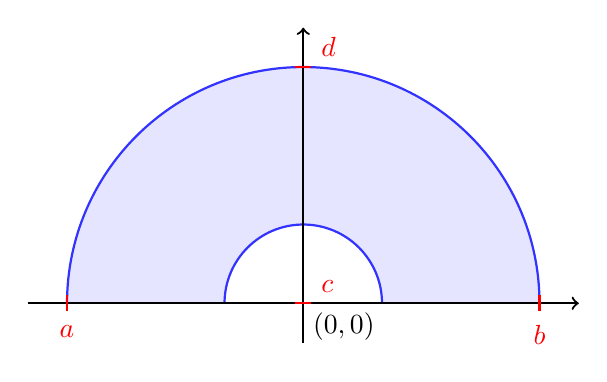
\begin{tikzpicture}
            \begin{scope}[thick]
                \clip (-3.5,0) rectangle (3.5,3.5);
                \path [draw=blue!80,fill=blue, fill opacity = 0.1,even odd rule] (0,0) circle (3) (0,0) circle (1);
            \end{scope}

            \begin{scope}
                \clip (-3.5,-0.5) rectangle (3.5,3.5);
                \draw[->,thick] (-3.5,0)--(3.5,0) node[right]{$x$};
                \draw[->,thick] (0,-3.5)--(0,3.5) node[above]{$y$};
            \end{scope}


            \draw[thick, red] (-3,-0.1)--(-3,0.1) node[below=0.25cm]{$a$};

            \draw[thick, red] (3,-0.1)--(3,0.1) node[below=0.25cm]{$b$};


            \draw[thick, red] (-0.1,0)--(0.1,0) node[above right]{$c$};

            \draw[thick, red] (-0.1,3)--(0.1,3) node[above right]{$d$};


            \draw (0,0) node[below right]{$(0,0)$};
        \end{tikzpicture}
    \end{center}
    \noindent As can be seen in the above diagram the given shape is a washer meaning that we expect the centroid to have an $x$-coordinate of $0$ because the area on either side will ``cancel''.
    The $y$-coordinate should be somewhere above $y=0$. The centroid is given by
    $$(\bar{x}, \bar{y})=\left(\frac{\int_{a}^{b} xf(x)\, dx}{\int_{a}^{b} f(x)\, dx}, \frac{\int_{c}^{d} yf(y)\, dy}{\int_{c}^{d} f(y)\, dy}\right)$$
    \noindent The area of the washer is actually just the area of the outer circle minus the area of the inner circle, meaning that the centroid can be found as follows
    $$(\bar{x}, \bar{y})=\left(\frac{\int_{-3}^{3} x\sqrt{9-x^{2}}\, dx - \int_{-1}^{1} x\sqrt{1-x^{2}}\, dx}{\int_{-3}^{3} \sqrt{9-x^{2}}\, dx - \int_{-1}^{1} \sqrt{1-x^{2}}\, dx}, \frac{\int_{0}^{3} y\sqrt{9-y^{2}}\, dy - \int_{0}^{1} y\sqrt{1-y^{2}}\, dy}{\int_{0}^{3} \sqrt{9-y^{2}}\, dy - \int_{0}^{1} \sqrt{1-y^{2}}\, dy}\right)$$
    \noindent Which is pretty nasty looking, but quickly simplifies nicely. Starting with the numerator of $\bar{x}$
    \begin{align*}
         & = \int_{-3}^{3} x\sqrt{9-x^{2}}\, dx - \int_{-1}^{1} x\sqrt{1-x^{2}}\, dx                                                      \\
         & = \int_{-3}^{3} x\sqrt{u}\, dx - \int_{-1}^{1} x\sqrt{w}\, dx \rightsquigarrow \text{ let } u=9-x^2 \text { and } w=1-x^2      \\
         & = -\frac{1}{2}\int_{-3}^{3} \sqrt{u}\, du + \frac{1}{2}\int_{-1}^{1} \sqrt{w}\, dw                                             \\
         & = \eval*{-\frac{1}{3}\left(9-x^2\right)^{\frac{3}{2}}}_{-3}^{3} + \eval*{\frac{1}{3}\left(1-x^2\right)^{\frac{3}{2}}}_{-1}^{1} \\
         & = 0                                                                                                                            \\
    \end{align*}

    \noindent Which means we don't have to care about integrating the denominator of $\bar{x}$ because it'll end up being $0$ as we expected. So, we currently sit knowing
    $$(\bar{x}, \bar{y})=\left(0, \frac{\int_{0}^{3} y\sqrt{9-y^{2}}\, dy - \int_{0}^{1} y\sqrt{1-y^{2}}\, dy}{\int_{0}^{3} \sqrt{9-y^{2}}\, dy - \int_{0}^{1} \sqrt{1-y^{2}}\, dy}\right)$$
    \noindent Now to integrate the numerator of $\bar{y}$
    \begin{align*}
         & = \int_{0}^{3} y\sqrt{9-y^{2}}\, dy - \int_{0}^{1} y\sqrt{1-y^{2}}\, dy                                                             \\
         & = \int_{0}^{3} y\sqrt{9-y^{2}}\, dy - \int_{0}^{1} y\sqrt{1-y^{2}}\, dy \rightsquigarrow \text{ let } q=9-y^2 \text { and } r=1-y^2 \\
         & = -\frac{1}{2}\int_{0}^{3} \sqrt{q}\, dq + \frac{1}{2}\int_{0}^{1} \sqrt{r}\, dr                                                    \\
         & = \eval*{-\frac{1}{3}\left(9-y^2\right)^{\frac{3}{2}}}_{0}^{3} + \eval*{\frac{1}{3}\left(1-y^2\right)^{\frac{3}{2}}}_{0}^{1}        \\
         & = \frac{26}{3}                                                                                                                      \\
    \end{align*}

    \noindent And the denominator of $\bar{y}$
    \begin{align*}
         & = \int_{0}^{3} \sqrt{9-y^{2}}\, dy - \int_{0}^{1} \sqrt{1-y^{2}}\, dy                                                                                                                                  \\
         & = \eval*{\frac{1}{2} \, \sqrt{-y^{2} + 9} y + \frac{9}{2} \, \arcsin\left(\frac{1}{3} \, y\right)}_{0}^{3} - \eval*{\frac{1}{2} \, \sqrt{-y^{2} + 1} y - \frac{1}{2} \, \arcsin\left(y\right)}_{0}^{1} \\
         & = 2\pi                                                                                                                                                                                                 \\
    \end{align*}

    \noindent Which I did partially with Sage because this assignment slipped my mind and I'm doing it kind of late on a Friday after a couple midterms :). Anyway, we now know that the centroid of the region $S$ is

    $$\left(0, \frac{13}{3\pi}\right)$$

    \begin{center}
        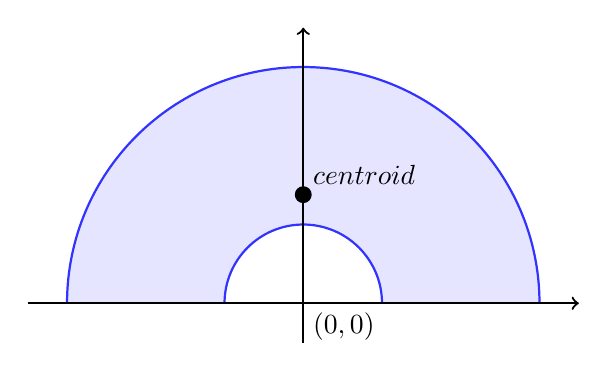
\begin{tikzpicture}
            \begin{scope}[thick]
                \clip (-3.5,0) rectangle (3.5,3.5);
                \path [draw=blue!80,fill=blue, fill opacity = 0.1,even odd rule] (0,0) circle (3) (0,0) circle (1);
            \end{scope}

            \begin{scope}
                \clip (-3.5,-0.5) rectangle (3.5,3.5);
                \draw[->,thick] (-3.5,0)--(3.5,0) node[right]{$x$};
                \draw[->,thick] (0,-3.5)--(0,3.5) node[above]{$y$};
            \end{scope}

            \draw (0,1.37934284012976) circle(0.1)node[above right]{$centroid$};
            \fill (0,1.37934284012976) circle(0.1);



            \draw (0,0) node[below right]{$(0,0)$};
        \end{tikzpicture}
    \end{center}

    \noindent at least I think, not much time to check as I've got to be up early tomorrow!

\end{soln}
\end{document}